\chapter{Redis: un veloce database in memoria}

\section{I database NoSQL}

Per database NoSQL, si intende ogni software atto alla memorizzazione strutturata dell'informazione
che, in rottura con l'usanza predominante già dagli anni '70, non utilizza lo \emph{Structured
Markup Langage} (SQL) per la manipolazione dei dati ivi contenuti. Nella maggioranza dei casi,
l'assenza del linguaggio SQL in realtà è solamente un sintomo di una importante differenza
architetturale: l'allontanamento dal paradigma di strutturazione in tabelle, record e relazione, e,
se vogliamo, anche dal modello E-R. Da questo punto di vista, il modo più corretto per identificare
l'insieme di questi software sarebbe quindi l'uso della locuzione "database non relazionali".

Il termine si è diffuso nel linguaggio popolare informatico dal 2010; si suole far
coincidere questa improvvisa attenzione con un omonimo workshop organizzato dalla società
californiana Rackspace (un fornitore di servizi cloud) in cui vennero analizzate
queste tecnologie a seguito del crescente interesse nell'ambiente della cosiddetta
\emph{Silicon Valley}.

I database NoSQL coprono quindi un ampio spettro di software completamente eterogenei
tra loro, adatti a scopi e situazioni diverse, con l'unico tratto a comune di non
utilizzare il modello relazionale.

\subsection{Tipologie di database}

Posto che una tassonomia esaustiva dei database NoSQL sarebbe impossibile in virtù
dell'ampiezza della definizione, ne proponiamo una \cite{corbellini} sufficiente a coprire le
principali tipologie e sottolinearne le differenze:

\begin{itemize}
	\medskip
	\item
	\textbf{Database Chiave-valore}: questi database si comportano come giganteschi array
	associativi distribuiti, nei quali dunque è possibile risalire ad un valore data la
	sua chiave univoca di riferimento. Vengono spessi offerti più spazi di chiavi
	a disposizione, e l'obiettivo di scala è molto elavato (fino a petabyte di dati
	e milioni di operazioni al secondo).

	\item
	\textbf{Database a famiglie di colonne}: questi database memorizzano i dati in un formato
	tabellare, ma senza garantire uno schema; in altre parole, ciascuna riga contiene
	una tupla in cui non tutte le colonne sono valorizzate (e, a seconda dei casi, la
	valorizzazione di una colonna può anche non avere un tipo specifico). In alcuni
	casi, sono presenti delle colonne speciali per identificatori univoci o timestamp,
	su cui costruire per lo meno indici parziali.

	\item
	\textbf{Database orientati al documento}: questi database memorizzano dati organizzati in
	"documenti", indicizzati con una chiave primaria. Ogni documento ha un suo spazio
	chiavi, e viene memorizzato secondo uno schema ben definito, ma più flessibile
	di quello utilizzato nelle tabella dei database relazionali; tipicamente infatti,
	è possibile aggiungere liberamente dati ad un documento, sebbene con determinati
	vincoli.

	\item
	\textbf{Database orientati ai grafi}: questi database sono pensati per memorizzare dati
	in formato tabellare, ma con relazioni multiple tra loro codificate in modo
	strutturato e preciso, in modo da formare dei grafi di relazioni, e con operazioni
	efficienti per effettuare l'analisi di questi grafi. I tipici casi d'uso sono
	quelli dove i dati presentano numerose relazioni di interconnessione, quali per
	esempio i dati di un social network.
\end{itemize}

Poiché Redis, oggetto di questa tesi, rientra pienamente nella prima categoria, sarà
questa che andremo ad analizzare con maggior dettaglio.


\subsection{I database chiave-valore}

Nei database chiave-valore, sia l'inserimento che la ricerca avviene tramite
la chiave primaria. Su questa chiave (tipicamente una stringa o array di byte),
viene applicata internamente una funzione hash che consente poi una strutturazione
in tabella dei dati con ricerca e inserimento efficiente. Per gestire il partizionamento
dei dato su più nodi, si utilizza normalmente una funzione hash consistente.

Per effettuare una ulteriore analisi più approfondita, è necessario suddividere
questi database in due grossi gruppi:

\begin{itemize}
	\medskip
	\item
	\textbf{Database chiave-valore in RAM}. Si tratta di database in cui l'intero dataset
	deve essere necessariamente contenuto nella RAM dei nodi del database
	(con eventuale distribuzione in più nodi). In questi database, dunque, tutte
	le operazioni principali vengono effettuate direttamente in RAM, e la persistenza
	su disco a volte è addirittura opzionale o eventuale (cioè non sempre consistente).
	Anche laddove viene richiesta una persistenza consistente, il database mantiene
	tutti i dati in RAM. Redis rientra in questa categoria.

	\item
	\textbf{Database chiave-valore su disco}. Al contrario dei precedenti, questi
	database seguono una struttura più classica. I dati vengono memorizzati infatti
	su disco fisso, mentre la RAM viene usata come memoria volatile per memorizzare
	parti di dati più frequentemente utilizzati, o indici sui dati stessi per un
	accesso rapido.
\end{itemize}

\section{Nascita dei database chiave-valore in RAM}

I database chiave-valore in RAM sono anche chiamati "cache distribuite", una sineddoche
che rimanda al tipo d'uso più comune, nato intorno alla metà degli anni 2000.

Con l'avvento dell'adozione di massa delle connessioni Internet in banda larga nei primi
anni 2000, i servizi su Internet hanno iniziato a sperimentare dei problemi di stabilità,
quando si trovavano a gestire alti picchi di traffico. Tali servizi, infatti, erano
comunemente implementati come un semplice servizio di tipo CGI, ospitato all'interno
del processo del webserver; in caso di traffico troppo elevato, l'unica soluzione possibile
era quella della cosidetta ``scalabilità verticale'', cioè eseguire il servizio su un
server più potente.

Il tema dei picchi di traffico, così alti e improvvisi da mettere fuori uso i siti,
era così dibattuto da avere anche un nome preciso: era comunemente chiamato ``Slashdot
effect'', dal nome del famoso portale Slashdot che, all'epoca, era molto visitato dagli
informatici di tutto il mondo. Il sito, ancora oggi operativo (sebbene non più così
visitato), pubblica una raccolta curata di notizie e link dedicati al mondo della tecnologia
e delle scienza. Accadeva spesso che alcuni siti, quando venivano pubblicati su Slashdot,
ricevessero una mole di visite troppo elevate che di fatto li mandava fuori uso; da qui
il nome.

In ottica di pura scalabilità verticale, uno dei modi più comuni per ottimizzare il software
applicativo è quello di aggiungere uno strato di cache in RAM, anteposta quindi al database, per
diminuire il numero di query che vengono fatte. Un esempio classico è la gestione delle sessioni:
quando un client comunica via HTTP con il server, inserisce sempre nelle richieste un cookie che
identifica univocamente la sessione dell'utente; tramite il cookie, il server può quindi riconoscere
la sessione e l'utente stesso. Tantissime richieste HTTP contengono un cookie di sessione, e di
conseguenza il server applicativo deve sempre risalire alla sessione prima ancora di entrare nel
merito della richiesta. Nei primi anni 2000, era normale memorizzare le sessioni nel database, ed
era dunque necessaria una query per ogni richiesta per recuperarla. Per ottimizzare la velocità del
software, era quindi opportuno cercare di limitare queste query, per esempio inserendo in una cache
in RAM le sessioni usate più di recente.

Il dibattito sulle soluzioni da adottare per ottenere la cosiddetta ``scalabilità orizzontale'',
cioè l'utilizzo di più di un server in parallelo come modo per aumentare le performance, si orientò
velocemente verso la replica indipendente dei server database e dei server applicativi, anteponendo
a questi ultimi dei bilanciatori di carico, che si occupassero di distribuire le connessioni
ingresso. Con questa architettura però, non era più possibile operare semplicemente una cache in RAM
dentro il server applicativo, poiché i bilanciatori di carico (a meno di complesse implementazioni)
non potevano facilmente garantire che ogni richiesta di una stessa sessione arrivasse allo stesso
server.

Per ovviare a questo inconveniente, nel 2003 nasce Memcached, scritto da Brad Fitzpatrick per
implementare la scalabilità orizzontale nel suo popolare gestore di blog LiveJournal. Memcached è di
fatto una tabella hash chiave-valore, raggiungibile via TCP con un semplice protocollo testuale. Le
operazioni sono stanzialmente due: GET e SET. È sufficiente qundi collegare tutti i server
applicativi ad un unico server Memcached (possibilmente sulla stessa rete fisica, beneficiando
quindi di una latenza molto bassa) perché possano condividere la stessa cache, aggiornando il codice
che prima utilizzava una tabella in RAM dentro il processo con una libreria che acceda alla stessa
tabella tramite chiamate TCP.

Memcached è il primo database NoSQL chiave-valore, ante-litteram, ed è oggi in uso presso alcuni
dei più popolari siti al mondo quali YouTube, Reddit, Facebook, Twitter, Tumblr, Wikipedia.


\section{Nascita di Redis}

Redis (acronimo di Remote Dictionary Service) è un database chiave-valore in RAM scritto
da Salvatore Sanfilippo e rilasciato per la prima volta nel 2008 sotto licenza BSD.

Redis nasce come costola di un progetto (ora defunto) chiamato "lloogg", un servizio di
analisi in tempo reale di log di siti. Originariamente, Sanfilippo aveva progettato
questo servizio  utilizzando MySQL come database primario per la memorizzazione dei
dati, ma presto questa scelta si era dimostrata errata, perché MySQL non raggiungeva le
performance desiderata in un contesto particolarmente intensivo dal punto di vista delle
scrittura come quello degli aggregatori di log \cite{nascita}.

Sanfilippo aveva necessità di memorizzare velocemente i dati in arrivo, e di eseguire
delle semplice query strutturate tipo "estrai gli ultimi N dati inseriti". Questo genere
di struttura non si applica bene al modello relazionale, in particolare perché l'ordine
di inserimento dei dati non viene preservato, e richiede quindi un'operazione di ordinamento
(o aggiornamento di un indice di ordinamento) ogni volta che un dato viene inserito.
Abbandonando il modello relazionale, invece, operazioni di questo genere si eseguono
in modo naturale ed efficiente con strutture dati quali le liste concatenate, ed è
proprio questa impedenza fondamentale tra modello relazionale e strutture dati primarie
alla base dell'architettura di Redis.

\section{Principali casi d'uso}


\section{Installazione}

Redis è stato scritto per funzionare su sistemi UNIX e supporta ufficialmente la
compilazione sotto Linux, macOS, OpenBSD, NetBSD e FreeBSD. Il codice è stato scritto
per essere compatibile anche con architetture a 32-bit, sebbene la versione a 64-bit
sia di gran lunga la più utilizzata in virtù della maggiore capacità di indirizzamento
di memoria.

La compilazione da codice sorgente è molto semplice: Redis è scritto nel linguaggio
ANSI C90, e le pochissime dipendenze a livello di librerie sono distribuite con il
codice sorgente stesso, quindi è sufficiente disporre sul sistema del compilatore GCC.
Una volta scaricato l'archivio di codice sorgente dalla \cite{pagina di scaricamento ufficiale}
o tramite \verb|git| dal \cite{repositorio ufficiale su GitHub}, è sufficiente lanciare il
comando \verb|make|. Questa l'intera sequenza:

\medskip
\begin{lstlisting}
$ git clone https://github.com/antirez/redis
$ cd redis
$ make
\end{lstlisting}

In alternativa, è possibile installare Redis da un pacchetto di distribuzione binario
presente nella maggior parte dei sistemi operativi. Per esempio, in un sistema Debian
o Ubuntu, è possibile eseguire il comando \verb|apt-get install redis-server|, mentre
su un sistema macOS si può utilizzare il gestore di pacchetti ``Homebrew'' tramite il
comando \verb|brew install redis|.

\section{Architettura}

Redis implementa un array associativo (tramite tabella hash) in cui le chiavi sono
stringhe, e i valori associati sono oggetti di vari tipi (stringhe o strutture dati).
Per comunicare con Redis, un client si deve connettere via TCP (la porta di default è la 6379) e
comunicare tramite un protocollo testuale di tipo master/slave. È possibile utilizzare
anche semplicemente \verb|telnet| per sperimentare, sebbene sia più comodo utilizzare il
client dedicato \verb|redis-cli| che offre il completamento intelligente dei comandi, la
storia dei comandi inseriti, e la formattazione leggibile dei risultati.

Come esempio, la seguente sessione mostra come scrivere e leggere un valore di tipo
stringa:

\medskip
\begin{lstlisting}
127.0.0.1:6379> SET abc provavalore
OK
127.0.0.1:6379> GET abc
"provavalore"
127.0.0.1:6379> GET abcd
(nil)
\end{lstlisting}

Il valore di ritorno visualizzato dalla console è fortemente tipizzato nel protocollo;
nei precedenti casi, il valore di ritorno è sempre una stringa (compreso l'ultimo
caso in cui la stringa è vuota, e viene dunque visualizzata come ``<nil>``).

Il comando \verb|DEL| può essere utilizzato per cancellare un oggetto di tipo
arbitrario:

\medskip
\begin{lstlisting}
127.0.0.1:6379> DEL abc
(integer) 1
127.0.0.1:6379> DEL notexisting
(integer) 0
\end{lstlisting}

In questo caso, il valore di ritorno è un intero, dal quale si può desumere se il comando
ha effettivamente cancellato un oggetto o meno. Gli errori sono anch'essi tipizzati in
modo separato. Per esempio, un comando inesistente restituisce un codice di errore:

\medskip
\begin{lstlisting}
127.0.0.1:6379> MYSQL
(error) ERR unknown command 'MYSQL'
\end{lstlisting}

Ogni chiave in Redis è una stringa (sequenza di byte) di lunghezza arbitraria; non è
necessario che sia stampabile, sebbene questo sia consigliabile per facilitare il
debugging. La funzione hash con la quale la stringa viene convertita in indice è
una semplice funziona polinomiale utilizzante un numero primo come base, 
comunemente chiamata djb2 \cite{djbhash}, dal nome del suo ideatore (Daniel J. Bernestein).

\section{Tipologie di oggetti memorizzabili}

Ogni oggetto memorizzato in Redis deve avere un tipo specifico, che viene serializzato
nella tabella e controllato ad ogni accesso. A livello di protocollo di comunicazione,
ogni comando opera su oggetti di uno specifico tipo; per esempio, i comandi \verb|SET|
e \verb|GET| visti nell'esempio precedente operano solamente su stringhe.

Oltre ai tipi base (stringhe, interi, numeri in virgola mobile), gli oggetti memorizzati
possono essere delle vere e proprio strutture dati quali liste, tabelle hash, insiemi
ordinati e così via. È proprio questa ricchezza in termini di strutture dati che caratterizza
Redis rispetto ad altri database della stessa tipologia.

Redis non prevede comandi espliciti di creazione di oggetti; è normalmente sufficiente
eseguire un comando di modifica di un oggetto (come per esempio il comando per aggiungere
un elemento ad un insieme) su una chiave non utilizzata per creare automaticamente una
struttura dati del tipo specificato, associandola alla chiave. Per esempio, il comando
\verb|SADD| viene utilizzato per aggiungere uno o più elementi ad un insieme; di
conseguenza, il comando \verb|SADD test1 elem1 elem2| creerà automaticamente un insieme 
associato alla chiave \verb|test1|, contenente i due elementi \verb|elem1| e \verb|elem2|.
Se \verb|test1| esistesse già nella base di dati ma fosse di tipo diverso (per esempio,
una lista), il comando \verb|SADD| ritornerebbe un errore (\verb|WRONGTYPE|).

Viceversa, come già visto nel precedente paragrafo, è previsto un comando di cancellazione
generale (\verb|DEL|) che rimuove la chiave e l'oggetto ad essa associato dal database,
qualunque sia il tipo dell'oggetto stesso.


\subsection{Stringhe}

Si tratta di sequenze di byte di lunghezza arbitraria. I comandi
più comuni per manipolarle sono, come visto, \verb|SET| e \verb|GET|, ma anche \verb|APPEND|
per concatenare, \verb|STRLEN| per leggere la lunghezza, o \verb|GETRANGE| per estrarre una
sottostringa.

\medskip
\begin{lstlisting}
127.0.0.1:6379> SET foo abcd
OK
127.0.0.1:6379> GET foo
"abcd"
127.0.0.1:6379> APPEND foo ef
(integer) 6
127.0.0.1:6379> STRLEN foo
(integer) 6
127.0.0.1:6379> GETRANGE foo 2 3
"cd"
\end{lstlisting}

Si noti come \verb|APPEND| ha restituito la nuova lunghezza della stringa, sfruttando
la disponibilità nel protocollo del valore di ritorno come modo per veicolare una
informazione possibilmente utile.

Le stringhe sono in realtà l'unico tipo primario supportato da Redis, ma vengono spesso usate come
tipo debole, cioè è possibile manipolarle come se fossero oggetti di altri tipi. Infatti, i comandi
\verb|INCR|, \verb|DECR|,  \verb|INCRBY| e \verb|DECRBY| ci permettono di interagire con oggetti di
tipo stringa che rappresentano degli interi in base 10:

\medskip
\begin{lstlisting}
127.0.0.1:6379> SET foo 123
OK
127.0.0.1:6379> STRLEN foo
(integer) 3
127.0.0.1:6379> INCR foo
(integer) 124
127.0.0.1:6379> STRLEN foo
(integer) 3
127.0.0.1:6379> DECRBY foo 24
(integer) 100
127.0.0.1:6379> GET foo
"100"
\end{lstlisting}

In questo esempio, alla chiave \verb|foo| è stato associato una stringa che contiene
la rappresentazione di un numero in base 10; il comando \verb|STRLEN| ci rassicura
che si tratta di una stringa di lunghezza 3. Nonostante questo, i comandi \verb|INCR|
e \verb|DECRBY| sono in grado di manipolare la stringa come se fosse un intero (e il
loro valore di ritorno infatti è di tipo intero). Al termine di queste operazioni
matematiche, il comando \verb|GET| conferma che si tratta sempre di una stringa.

Allo stesso modo, viene fornito un supporto molto blando per i numeri in virgola
mobile tramite il comando \verb|INCRBYFLOAT|.

Una possibilità più avanzata è quella di considerare la stringa come un array di bit
utilizzando i comandi \verb|BITCOUNT|, \verb|SETBIT| e \verb|GETBIT| per lavorare
su ciascun bit.

\subsection{Liste}

In Redis, le liste sono strutture dati assimilabili, come complessità computazionale,
alle normali liste con puntatore doppio; i valori contenuti nella lista sono stringhe.
L'accesso al primo e all'ultimo elemento ha una complessità di O(1), mentre
l'accesso all'elemento N richiede O(N). I comandi principali per manipolare una
lista sono i seguenti:

\begin{itemize}
	\medskip
	\item \textbf{LPUSH}. Aggiunge un elemento in cima alla lista.
	\item \textbf{RPUSH}. Aggiunge un elemento in fondo alla lista.
	\item \textbf{LPOP}. Rimuove un elemento dalla cima della lista.
	\item \textbf{RPOP}. Rimuove un elemento dal fondo della lista.
	\item \textbf{LLEN}. Restituisce la lunghezza della lista.
	\item \textbf{LINDEX}. Restituisce l'elemento K-esimo della lista.
	\item \textbf{LRANGE}. Restituisce tutti gli elementi all'interno di un range di indici.
	\item \textbf{LSET}. Modifica l'elemento K-esimo della lista.
	\item \textbf{LINSERT}. Inserisce un elemento prima o dopo un elemento pivot.
\end{itemize}

Qui si può vedere una sessione interattiva di esempio di uso di una lista:

\medskip
\begin{lstlisting}
127.0.0.1:6379> RPUSH mylist mickey minnie goofy donald
(integer) 4
127.0.0.1:6379> LINDEX mylist 0
"mickey"
127.0.0.1:6379> LINDEX mylist 1
"minnie"
127.0.0.1:6379> LPOP mylist
"mickey"
127.0.0.1:6379> LLEN mylist
(integer) 3
127.0.0.1:6379> LINSERT mylist AFTER goofy walt
(integer) 4
127.0.0.1:6379> LRANGE mylist 0 5
1) "minnie"
2) "goofy"
3) "walt"
4) "donald"
\end{lstlisting}

Si noti che non è necessario inizializzare la lista in nessun modo: il primo riferimento alla chiave
\verb|mylist| tramite un comando \verb|RPUSH| (che opera esclusivamente su liste) è sufficiente
per creare dinamicamente l'oggetto di tipo giusto.

\subsection{Tabelle hash}

Una tabella hash consente di memorizzare una serie di coppie di stringhe (denominate ``campo'' e
``valore''), associandole ad una chiave del database; questo consente quindi di serializzare dei
semplici oggetti, sebbene non sia possibile avere tipologie più complesse di dati.

Un esempio di uso di tabella hash è la memorizzazione delle informazioni sugli utenti di un
applicativo; è possibile infatti utilizzare come chiave una stringa composta da un prefisso (per
esempio \verb|user|), seguito dall'ID univoco (chiave primaria) dell'utente, per esempio un intero
progressivo, opzionalmente divis da un separatore per leggibilità (\verb|user:88|). All'interno
della tabella, i campi sono i nomi degli attributi che si vuole memorizzare (\verb|nome|,
\verb|cognome|, ecc.), associati ai relativi valori.

Si noti che non esiste nessun controllo d'integrità che ci assicuri che le tabelle associate a tutti
gli utenti (tutte le chiavi con prefisso \verb|user|, nel nostro esempio) siano consistenti tra loro
e dunque popolate dai medesimi campi; così come non è possibile verificare la tipizzazione dei
campi, poiché i valori sono esclusivamente di tipo stringa e dunque senza tipo. Se dunque è
necessaria uniformità, l'onere è lasciato al client.

I comandi principali sono i seguenti, caratterizzata dal prefisso \verb|H|:

\begin{itemize}
	\medskip
	\item \textbf{HSET}. Aggiunge un campo alla tabella.
	\item \textbf{HGET}. Legge il valore di un campo della tabella.
	\item \textbf{HDEL}. Cancella un campo dalla tabella.
	\item \textbf{HEXISTS}. Verifica se un campo è presente nella tabella.
	\item \textbf{HLEN}. Restituisce il numero di campi presenti nella tabella.
	\item \textbf{HGETALL}. Restituisce tutte i campi e tutti i valori nella tabella.
	\item \textbf{HMGET} e \textbf{HMSET}. Rispettivamente come \verb|HGET| e \verb|HSET| ma operano
	su campi multipli.
	\item \textbf{HKEYS} e \textbf{HVALS}. Restituiscono rispettivamente tutti i campi e tutti i
	valori nella tabella.
\end{itemize}

Qui si può vedere una sessione interattiva di esempio di uso di una tabella hash:

\medskip
\begin{lstlisting}
127.0.0.1:6379> HSET user:88 name giovanni
(integer) 1
127.0.0.1:6379> HMSET user:88 surname bajo age 38
OK
127.0.0.1:6379> HLEN user:88
(integer) 3
127.0.0.1:6379> HGET user:88 surname
"bajo"
127.0.0.1:6379> HGETALL user:88
1) "name"
2) "giovanni"
3) "surname"
4) "bajo"
5) "age"
6) "38"
127.0.0.1:6379> HKEYS user:88
1) "name"
2) "surname"
3) "age"
127.0.0.1:6379> HVALS user:88
1) "giovanni"
2) "bajo"
3) "38"
127.0.0.1:6379> HEXISTS user:88 name
(integer) 1
127.0.0.1:6379> HEXISTS user:88 giovanni
(integer) 0
\end{lstlisting}

Come si può vedere, la tabella hash è creata dinamicamente al primo uso, e non è necessario
dimensionarla in alcun modo; Redis implementa in modo efficiente le tabelle hash e le ridimensiona
automaticamente al crescere degli elementi contenuti, mantentendo un fattore massimo di riempimento
che garantisce una buona velocità di accesso.

\subsection{Insiemi}

Un insieme in Redis è una sequenza non ordinata di stringhe univoche, associate ad una chiave del
database. È possibile compiere le operazioni base quali l'aggiunta di una stringa, la rimozione di
una stringa, il conteggio della cardinalità, la verifica della presenza di una stringa, l'estrazione
di una stringa scelta casualmente tra quelle presenti. Inoltre, sono previste anche operazioni che
coinvolgono più di un insieme, quali il calcolo dell'intersezione, dell'unione, della differenza.

Riprendendo il precedente esempio di tabella hash contenente gli utenti, un applicativo potrebbe
voler memorizzare all'interno di un insieme l'elenco degli utenti che soddisfano una determinata
proprietà, per esempio tutti coloro che hanno effettuato almeno un pagamento, o coloro che hanno
aggiornato all'ultima versione dell'applicativo. In questo caso, si potrebbe quindi creare due
insiemi, associati alle chiavi \verb|paying_users| e \verb|updated_users|, e inserirvi gli ID degli
utenti (\verb|88|, \verb|4|, \verb|37|, ecc.). Sarebbe poi possibile effettuare rapide operazioni di
controllo di appartenenza, oppure di differenza (ottenendo quindi l'elenco degli utenti paganti che
non hanno aggiornato all'ultima versione, in modo da poter per esempio inviare loro una email di
sollecito).

Nei database relazionali, queste operazioni sono tipicamente possibile tramite delle query SQL, che
il database rende efficente tramite indici. Allo stesso modo, in questo esempio abbiamo utilizzato
un insieme come indice esterno di una tabella, dovendolo però aggiornare manualmente.

Questi sono i principali comandi che Redis prevede per gli insiemi, caratterizzati dal prefisso
\verb|S|:

\begin{itemize}
	\medskip
	\item \textbf{SADD}. Aggiunge una stringa ad un insieme.
	\item \textbf{SREM}. Rimuove una stringa da un insieme.
	\item \textbf{SISMEMBER}. Controlla se una stringa è presente in un insieme.
	\item \textbf{SMEMBERS}. Elenca tutte le stringhe contenute nell'insieme.
	\item \textbf{SRANDMEMBER}. Restituisce una o più stringhe scelte casualmente tra quelle
	presenti.
	\item \textbf{SPOP}. Come ``SRANDMEMBER'', ma rimuove le stringhe scelte dall'insieme.
	\item \textbf{SUNION}. Restituisce l'unione tra due o più insiemi.
	\item \textbf{SINTER}. Restituisce l'interesezione tra due o più insiemi.
	\item \textbf{SDIFF}. Restituisce la differenza tra un insieme e uno o più altri insiemi.
	\item \textbf{SUNIONSTORE}, \textbf{SINTERSTORE}, \textbf{SDIFFSTORE}: Come i comandi
	precedenti, ma il risultato dell'operazione viene memorizzato in Redis in una nuova chiave
	specificata, e viene restituita solo la cardinalità del risultato.
\end{itemize}

Qui si può vedere una sessione interattiva di esempio di uso degli insiemi:

\medskip
\begin{lstlisting}
127.0.0.1:6379> SADD paying_users 88 37 4 66
(integer) 4
127.0.0.1:6379> SADD paying_users 37 111
(integer) 1
127.0.0.1:6379> SISMEMBER paying_users 111
(integer) 1
127.0.0.1:6379> SREM paying_users 37
(integer) 1
127.0.0.1:6379> SCARD paying_users
(integer) 4
127.0.0.1:6379> SISMEMBER paying_users 37
(integer) 0
127.0.0.1:6379> SADD updated_users 12 4 66
(integer) 3
127.0.0.1:6379> SDIFF paying_users updated_users
1) "88"
2) "111"
127.0.0.1:6379> SINTER paying_users updated_users
1) "4"
2) "66"
\end{lstlisting}

Anche in questo caso, non è stato necessario allocare o dimensionare le strutture dati: al primo
accesso, esse vengono create automaticamente, e si dimensionano in modo dinamico durante l'uso.

\subsection{Insiemi ordinati}

Un insieme ordinato è una sequenza di stringhe univoche, ordinate secondo un valore associato
chiamato ``punteggio''. Ogni inserimento di una stringa viene effettuato specificando il suo
punteggio (aggiornando quindi un eventuale puntegggio già esistente), e la struttura dati effettua
l'inserimento (o lo spostamento) nel modo giusto per mantenere l'ordinamento. In questo modo, è
possibile effettuare sia operazioni di tipo insiemistico (controllo appartenenza, aggiunta,
rimozione, unioni, intersezioni), sia operazioni che lavorano su intervalli di stringhe all'interno
della sequenza (per esempio, delimitandone gli estremi per punteggio).

Il punteggio deve essere specificato come un valore decimale con virgola, e le stringhe vengono
ordinate secondo l'ordinamento crescente. In caso due stringhe abbiano lo stesso punteggio, si
utilizza l'ordinamento lessicografico tra le stringhe stesse per decide l'ordine. In virtù di
questa proprietà, è comune utilizzare un insieme ordinato in cui tutti i valori hanno un medesimo
punteggio (di solito 0), utilizzando quindi le stringhe stesse per l'ordinamento, e ottenendo di
fatto l'equivalente di una lista di stringhe univoche ordinate alfabeticamente.

Come precedentemente accennato, è possibile estrarre sotto-sequenze dell'insieme ordinato tramite
alcuni comandi che lavorano su intervalli ordinati di stringhe. Secondo il principio di massima
flessibilità, ci sono tre diversi tipi di intervalli che possono essere specificati: intervallo di
punteggio (es: estrai tutte le stringhe i cui punteggi sono compresi tra 10 e 20), intervallo di
posizione (es: estrai le prime 10 stringhe secondo l'ordinamento attuale), oppure intervallo
lessicografico (es: estrai tutte le stringhe che iniziano con la lettera K); quest'ultimo tipo di
intervallo è in realtà correttamente definito solo quando il punteggio di tutte le stringhe è lo
stesso, e cioè quando la struttura dati sta di fatto già ordinando alfabeticamente, ma l'esistenza
comandi dedicati a questa modalità sottolinea proprio la flessibilità di questa struttura dati.

Questi sono i principali comandi esistenti, identificati dal prefisso \verb|Z|:

\begin{itemize}
	\item \textbf{ZADD}: aggiunge una o più stringhe all'insieme ordinata, associandole ad un
	punteggio. Se le stringhe esistono già, il punteggio viene aggiornato al valore specificato. Il
	comando prevede anche una serie di opzioni avanzate per cambiare il comportamento di default in
	caso di stringa già esistente.
	\item \textbf{ZINCRBY}: si comporta come \verb|ZADD|, ma in caso di stringa esistente il
	punteggio viene modificato in modo relativo, sommando cioè il valore specificato invece che
	sostituirlo.
	\item \textbf{ZREM}: rimuove una o più stringhe dall'insieme.
	\item \textbf{ZSCORE}: ritorna il punteggio associato ad una stringa, e può essere usato anche
	come test di appartanenza.
	\item \textbf{ZCARD}: ritorna la cardinalità dell'insieme, cioè il numero di stringhe
	contenute.
	\item \textbf{ZINTERSTORE}, \textbf{ZUNIONSTORE}: come le controparti per gli insieme,
	effettuano le operazioni (rispettivamente) di unione e intersezione, memorizzando il risultato
	in un nuovo insieme ordinato. Il punteggio ottenuto è la somma dei punteggi specificati negli
	insiemi di origine, ma è possibile specificare una funzione di aggregazione diversa (media,
	minimo o massimo), oltre che applicare dei pesi (fattori moltiplicativi) ai punteggi.
	\item \textbf{ZRANGE}: resituisce gli elementi all'interno dell'intervallo specificato come
	indice di sequenza. Per esempio, specificando come intervallo inclusivo \verb|0 4|, si
	ottengono i primi 5 elementi, cioè i 5 elementi con minor punteggio attualmente presenti
	nell'insieme. È possibile usare gli indici negativi per fare riferimento alla fine della
	sequenza (per esempio, \verb|-1| indica l'elemento con punteggio più alto).
	\item \textbf{ZRANGEBYSCORE}: restituisce gli elementi all'interno dell'intervallo specificato
	come punteggi. Per esempio, specificando come intervallo \verb|100.2 100.8|, si ottengono tutti
	gli elementi i cui punteggi sono compresi tra 100.2 e 100.8. Gli estremi dell'intervallo
	possono essere specificati come aperti o chiusi. È possibile inoltre specificare un numero
	massimo di elementi restituiti per evitare trasferimenti troppo pesanti (consentendo quindi la
	paginazione).
	\item \textbf{ZRANGEBYLEX}: restituisce gli elementi all'interno dell'intervallo specificato
	come prefissi lessicografici. Per esempio, specificando come intervallo \verb|AZ C|, si
	ottengono tutti gli elementi che seguono lessicograficamente la stringa ``AZ'' e precedono la
	stringa ``C''. Come per il comando precedente, è possibile specificare se gli estremi
	dell'intervallo sono aperti o chiusi, e indicare un limite massimo agli elementi restituiti.
	Come già descritto, questo comando funziona correttamente solo con insiemi ordinati in cui
	tutti gli elementi hanno lo stesso punteggio.
	\item \textbf{ZREVRANGE}, \textbf{ZREVRANGEBYSCORE}, \textbf{ZREVRANGEBYLEX}: simili ai
	precedenti comandi, ma considerano l'insieme ordinato al contrario, cioè in ordine decrescente
	di punteggio.
	\item \textbf{ZREMRANGEBYRANK}, \textbf{ZREMRANGEBYSCORE}, \textbf{ZREMRANGEBYLEX}: simili ai
	precedenti comandi, ma rimuovono gli elementi all'interno degli intervalli specificati invece
	che restituirli.
\end{itemize}

Anche gli insiemi ordinati, come gli insiemi, si prestano molto bene a creare indici manuali,
sempre ordinati, su cui effettuare poi operazioni di estrazione e ricerca. Vista la flessibilità
della struttura dati, indichiamo alcuni possibili scenari applicativi.

\begin{itemize}
	\medskip

	\item Un esempio di struttura dati facilmente rappresentabile tramite insieme ordinato è una
	coda con priorità. Supponiamo per esempio di dover memorizzare un elenco di azioni da eseguire
	nel futuro, assieme con l'istante temporale al quale l'azione deve essere eseguita. Al momento
	di inserire un'azione, si può creare un nuovo elemento in una tabella hash (\verb|HSET|)
	utilizzando un ID progressivo conservato in una chiave (\verb|INCR|), memorizzando così tutto
	il dettaglio dell'azione da eseguire (tipologia, parametri, condizioni di errore). Dopodiché,
	si inserisce l'ID dell'azione in un insieme ordinato (\verb|ZADD|), utilizzando come punteggio
	il timestamp UNIX a cui si dovrà eseguire l'azione. Successivamente, in polling, è possibile
	estrarre tutte le azioni scadute (cioè il cui timestamp è inferiore all'attimo corrente,
	tramite \verb|ZRANGEBYSCORE|) e processarle; via via che ciascuna azione termina l'esecuzione,
	può essere rimossa dall'insieme (\verb|ZREM|).

	\item Supponiamo di voler creare un sistema di loyalty per un e-commerce, basato sulla spesa 
	effettuata da ciascun utente. Ogni volta che un utente effettua un acquisto, possiamo
	memorizzato nell'insieme ordinato l'ID dell'utente aggiungendo l'importo del carrello
	(\verb|ZINCR|); non è necessario gestire in modo diverso il primo acquisto, perché \verb|ZINCR|
	funziona anche se l'elemento non è ancora presente. Se vogliamo contattare tutti gli utenti che
	hanno speso più di €1000 sul nostro e-commerce, possiamo utilizzare \verb|ZRANGEBYSCORE|
	specificando l'intervallo \verb|1000.00 +inf| per estrarre gli ID. In alternativa, supponendo
	di voler premiare i 100 utenti che hanno speso di più, possiamo estrarre i loro ID con
	\verb|ZREVRANGE| usando l'intervallo \verb|0 99| (essendo l'insieme in ordine crescente,
	dobbiamo usare \verb|ZREVRANGE| per estrarre facilmente gli elementi con punteggio più grosso).
\end{itemize}

Qui si può vedere una sessione interattiva di esempio di uso degli insiemi ordinati:

\medskip
\begin{lstlisting}
127.0.0.1:6379> ZADD test 10 a 20 b 30 c
(integer) 0
127.0.0.1:6379> ZCARD test
(integer) 3
127.0.0.1:6379> ZSCORE test b
"20"
127.0.0.1:6379> ZRANGE test 0 0
1) "a"
127.0.0.1:6379> ZRANGE test 0 10
1) "a"
2) "b"
3) "c"
127.0.0.1:6379> ZREVRANGE test 0 0
1) "c"
127.0.0.1:6379> ZRANGEBYSCORE test 15 25
1) "b"
127.0.0.1:6379> ZINCRBY test 20 b
"40"
127.0.0.1:6379> ZRANGEBYSCORE test 15 25
(empty list or set)
\end{lstlisting}


\subsection{HyperLogLog}

\section{Velocita}

(benchmark)
(segnalare problema del rountrip di rete)


\section{Transazioni}

(atomicità, non performance perché sono necessari X roundtrip)


\section{Pipelining}

Come dettagliato nella precedente sessione, le prestazioni ottenute nell'utilizzo di Redis sono
fortemente influenzate dalla velocità di rete. Sebbene le migliori pratiche di installazione in
ambiente di produzione consigliano di posizionare rete su un server (o gruppi di server) fisicamente
vicini al server dove girare l'applicazione client, in popolari ambienti cloud come Amazon Web
Services è possibile misurare latenze anche nell'ordine di 50 ms se si considerano misure al
99-esimo percentile, sebbene con valori mediani stabilmente sotto il millisecondo
\cite{aws-latency}.

L'utilizzo di transazioni, sebbene utile per introdurre il concetto di atomocità di esecuzione,
non migliora la latenza poiché ogni comando viene inviato separatamente e necessita quindi di un 
roundtrip (ai quali si sommano addirittura i due roundtrip richiesti da \verb|MULTI| e \verb|EXEC|).

Per arginare questo problema, Redis consente il \emph{pipelining}, una tecnica molto comune, 
utilizzata anche da altri protocolli di tipo master-slave come HTTP, IMAP e POP3. Dopo l'invio 
di un comando, il client può immediatamente inviarne un secondo senza necessariamente leggere
la risposta del primo dalla rete; il server infatti è in grado di mantenere memorizzate le risposte
dei comandi (memoria permettendo) indefinitamente, in attesa che il client le richieda. Dovendo
quindi eseguire una sequenza predeterminata di comandi, come nel caso di una transazione, il
pipelining risulta particolarmente comodo perché l'intera transazione (comprensiva dei delimitatori
\verb|MULTI| e \verb|EXEC|) può essere inviata consecutivamente, praticamente senza attese.

\begin{figure}
	\centering
		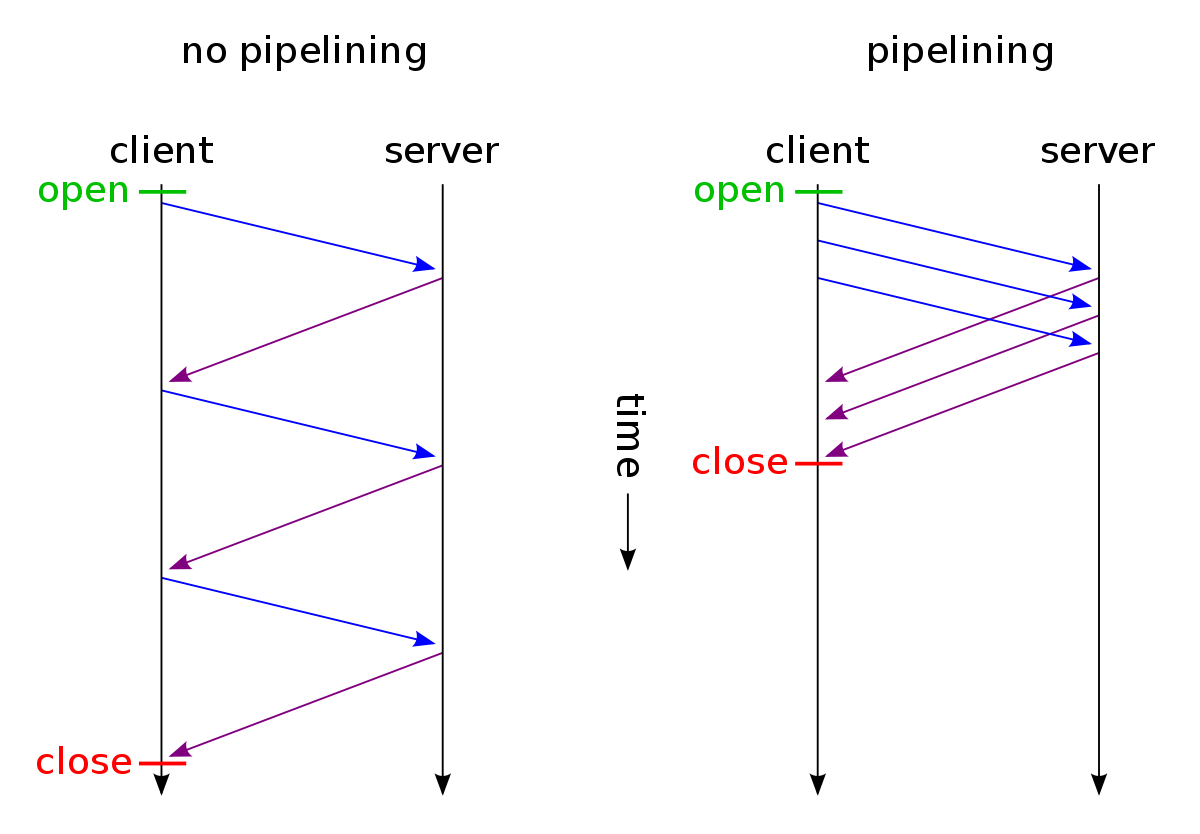
\includegraphics[width=0.8\textwidth]{pipelining}
	\caption{Diagramma di protocollo che mostra l'utilizzo del pipelining per diminuire la latenza
	di rete \emph{(Fonte: Wikipedia)}}
\end{figure}

Si noti che, se si è interessati ad ottenere la massima performance, è consigliabile anche
disattivare l'algoritmo di Nagle, ed utilizzare le opzioni \verb|TCP_NODELAY| e \verb|TCP_CORK| per
gestire manualmente il buffering \cite{tcp-cork}. Molte librerie client Redis per i principali
linguaggi di programmazione si occupano di questi dettagli automaticamente; si veda a titolo di
esempio i sorgenti della libreria \verb|redis-py| \cite{tcp-cork-redispy}.

\section{Stored procedure in LUA}

Il \emph{pipelining} non è però in grado di essere sempre utilizzato: per esempio, può essere
necessario verificare che un comando abbia successo prima di procedere al successivo; oppure
può essere necessario utilizzare il valore restituito da un comando per definire il parametro 
di un comando successivo. In questi casi, è necessario quindi introdurre un nuovo roundtrip di
rete per leggere la risposta, processarla, e inviare il successivo comando.

Esattamente come nel caso dei comuni database SQL, Redis consente di risolvere in modo più completo
il problema della latenza di rete tramite le cosidette \emph{stored procedure}: il programmatore può
inviare al database un programma speciale, che viene memorizzato per usi successivi, ed eseguirlo
poi successivamnete; questo programma può quindi effettuare più operazioni in successione, oltre che
utilizzare istruzioni per controllo di flusso, pagando, in termini di latenza, un solo roundtrip di
rete. Inoltre, specialmente nel caso in cui sia necessario effettuare delle funzioni di aggregazione
di dati (es: calcolo di una media), non è necessario trasferire via rete tutti i dati, ma solamente
il risultato.

Invece che utilizzare un linguaggio di programmazione progettato ad-hoc (come per esempio il
linguaggio PL/pgSQL \cite{plpgsql} utilizzato dal famoso database PostgreSQL), Redis utilizza un
linguaggio già esistente: LUA \cite{lua}. LUA è un linguaggio di scripting, tipato dinamicamente,
normalmente eseguito tramite un interprete molto efficiente e compatto, facilmente adatto
all'integrazione (embedding). Già dai primi anni 2000, ha ottenuto molto popolarità nell'industria
videoludica come linguaggio di scripting, proprio in virtù del profilo di performance e compatezza
che lo rendeva utilizzabile anche all'interno di console con processori non troppo potenti e
quantitativi di memoria limitati (si pensi per esempio alla Sony Playstation 2, che era comandata da
un processore MIPS R5900 a 300Mhz con 32Mb di RAM), ed è stato utilizzato all'interno di successi
quali Angry Birds \cite{lua-angry} o World of Warcraft \cite{lua-wow}.

Supponiamo di voler scrivere una stored procedure che calcoli un dato statistico aggregato; per
esempio, dato un insieme ordinato \verb|paying-users| ln cui le stringhe sono gli ID degli utenti
di un sistema, e il punteggio associato è il totale speso dall'utente nell'applicazione, vogliamo
calcolare qual è la media di spesa degli utenti ``premium'', cioè che hanno speso più di €1000. 
Per fare questo, è necessario estrarre prima la lista degli utenti premium tramite il comando
\verb|ZRANGEBYSCORE|, e poi iterare in questa lista calcolando il valore medio. L'utilizzo di una
stored precedure ci consente di fare questo senza trasferire sulla rete le informazioni relative
a tutti gli utenti premium, che potrebbero essere migliaia o anche più. Il sorgente LUA che
implementa questo semplice algoritmo è mostrato nel seguente listato:

\medskip
\lstinputlisting{code/zsetaverage.lua}

Come si nota, il sorgente può essere parametrizzato tramite dei parametri di tipo chiave/valore
che verranno passati al momento dell'utilizzo; in questo caso, si è scelto di passare come parametro 
la chiave dell'insieme ordinato da utilizzare, e la soglia minima di spesa, rendendo così lo script 
più generico e flessibile. Le chiavi dei parametri (accessibili tramite l'array \verb|KEYS|) non
sono invece utilizzate.

Per provare ad eseguire lo script durante la fase di sviluppo, è consigliabile l'utilizzo
dell'opzione \verb|--eval| del comando \verb|redis-cli|:

\medskip
\begin{lstlisting}
$ redis-cli
127.0.0.1:6379> ZADD paying_users 1000 a 2000 b 3000 c 3000 d 250 e
(integer) 5
$ redis-cli --eval zsetaverage.lua k t , paying_users 1000
(integer) 2250
$ redis-cli --eval zsetaverage.lua k t , paying_users 2000
(integer) 2666
\end{lstlisting}

Si noti che abbiamo passato 2 parametri: il primo con chiave \verb|k| e valore \verb|paying_users|;
il secondo con chiave \verb|t| e valore \verb|1000| (o \verb|2000|). L'identificatore \verb|,|
separara l'elenco delle chiavi (che non sono utilizzate dal nostro script) dall'elenco dei valori.

L'uso in produzione invece richiede due fasi: prima, lo script viene caricato nel database
come stored procedure tramite il comando \verb|SCRIPT LOAD|, che restituisce un ID univoco. 
Successivamente, lo script può essere eseguito richiamandolo tramite il suo ID, e specificando 
i parametri, con il comando \verb|EVALSHA|.

In questo caso, la sequenza è la seguente:

\medskip
\begin{lstlisting}
127.0.0.1:6379> SCRIPT LOAD "-- zsetaverage.lua: calcola la media di spesa degli utenti paganti sopra\n-- una certa soglia.\n--\n-- Argomenti:\n--     ARGV[1] - chiave dell'insieme ordinato\n--     ARGV[2] - soglia di spesa\n\n-- Estrae tutti gli utenti con un punteggio maggiore a quello specificato.\n-- L'opzione WITHSCORES dice a redis di tornare non solo le stringhe\n-- dell'insieme ordinato (quindi gli ID degli utenti) ma anche i \n-- punteggi associati.\n-- matches sara' quindi un array contenente in sequenza ID1, SCORE1, ID2, SCORE2, ecc.\nlocal matches = redis.call('ZRANGEBYSCORE', ARGV[1], ARGV[2], '+inf', 'WITHSCORES')\n\nlocal total = 0\n\n-- Attraversa l'array a partire dal secondo elemento, fino alla sua lunghezza,\n-- con passo 2. In questo modo ad ogni passo indirizziamo direttamente i punteggi\n-- saltando gli ID\n-- Si noti che in LUA il primo elemento di un array ha indice 1\nfor idx=2, #matches, 2 do\n    total = total + tonumber(matches[idx])\nend\n\n-- Calcola la media\nreturn total / (#matches / 2)\n"
"c8fe4ea641681f744e517b52002266ca7b4e4cdf"
127.0.0.1:6379> EVALSHA c8fe4ea641681f744e517b52002266ca7b4e4cdf 2 k t paying_users 1000
(integer) 2250
127.0.0.1:6379> EVALSHA c8fe4ea641681f744e517b52002266ca7b4e4cdf 2 k t paying_users 2000
(integer) 2666
\end{lstlisting}

Il comando \verb|EVALSHA| riceve come argomento l'ID dello script, il numero di parametri, e poi
in sequenza tutte le chiavi (non utilizzate nel nostro esempio) e tutti i valori. 

Si noti che l'ID dello script è in realtà il suo hash crittografico ottenuto tramite l'algoritmo
SHA-1; questo vuol dire che caricando più volte lo stesso script si otterrà sempre lo stesso valore
ed è inoltre possibile precalcolare l'ID che uno script avrà, per semplicità di implementazione.

\section{Utilizzo come cache}

(TTL e timeout)




\section{Concorrenza}

Coerentemente con la sua archiettura orientata alla semplicità e al minimalismo, Redis ha un
supporto primitivo ma efficace per la concorrenza, che è basato sulla serializzazione delle
operazioni. La scelta è dovuta al fatto che l'esecuzione di ciascun comando è (nella maggior parte
dei casi) molto veloce anche con grossi dataset, come si è visto, trattandosi di operazioni dirette
su specifiche strutture dati completamente conservate in memoria, senza necessità di interrogare o
aggioranare indici, né effettuare I/O di alcun tipo.

All'interno di ciasuna connessione TCP, il protocollo proibisce di eseguire comandi in parallelo,
cioè il client deve necessariamente attendere il risultato di un comando prima di poter inviare il
comando successivo (con l'unica eccezione dell'esecuzione di una transazione, che però come abbiamo
visto si configura di fatto come un unico comando inviato a livello di protocollo).

Viceversa, per quanto concerne comandi inviati da più clienti (e quindi tramite più connessioni) in
parallelo, Redis provvede a serializzarli tra loro in automatico poiché il codice del server si
basa su un singolo thread di esecuzione, e gestisce l'accesso ai socket in parallelo tramite
programmazione asincrona e accesso I/O non bloccante, appoggiandosi a primitive quali \verb|select| 
\cite{select}, \verb|epoll| \cite{epoll} o \verb|kqueue|.

Questa architettura rende il codice di Redis più semplice e veloce, perché non è necessario
acquisire né lock granulari nell'accesso ai singoli oggetti e strutture dati, né un lock globale
per serializzare gli accessi tra diversi thread in carico di gestire ciascuna connesione. L'uso di
lock quale per esempio un ``mutex'' implementato dalla libreria \verb|pthread| avrebbe un impatto non
solo a livello di semplicità di codice sorgente, ma anche di performance, poiché acquisire un lock
impiega un tempo non trascurabile rispetto alla reale esecuzione dell'operazioni richiesta, anche
nel caso in cui non è conteso.

\section{Persistenza}




